In this chapter we review the results obtained through out this work and obtain phyisicaly relevant quantities from our simulations and analytical computations. 

Throughout this work we have explored three different setups. Firstly we explored the case where there is no chemical reaction at the interface. This is the case of normal electrolytes under no external electric field. Secondly we studied the case where current is imposed through the electrolyte solution and therefore reaction is driven by this current. 

Lastly we studied the case where the reaction takes the form of Langmuir isotherm in the limiting case where the constant $K_{eq}S_T << 1$. 

An interesting parameter extractable from our models is the relaxation time, or the time it takes the system to reach steady state. Also we are interested in finding how the electric field at the surface varies with bulk concentrations and the electrolytic cell's potential.  We'll first analyze steady state solutions and then we'll move on to the dynamical system.



\section{Comparing Numeric An Analytic Results In Steady State Regime}

Fig. \ref{fig:comparison} shows the comparison between the numeric and analytic results. This results are obtained by numerically evaluation system of equations \ref{eq:nernst-planck} and perturvatively finding solutions up to first order on a forced current setup as shown in \ref{eq:first-order-system}



\begin{figure}[htbp]
\begin{subfigure}{.5\linewidth}
\centering
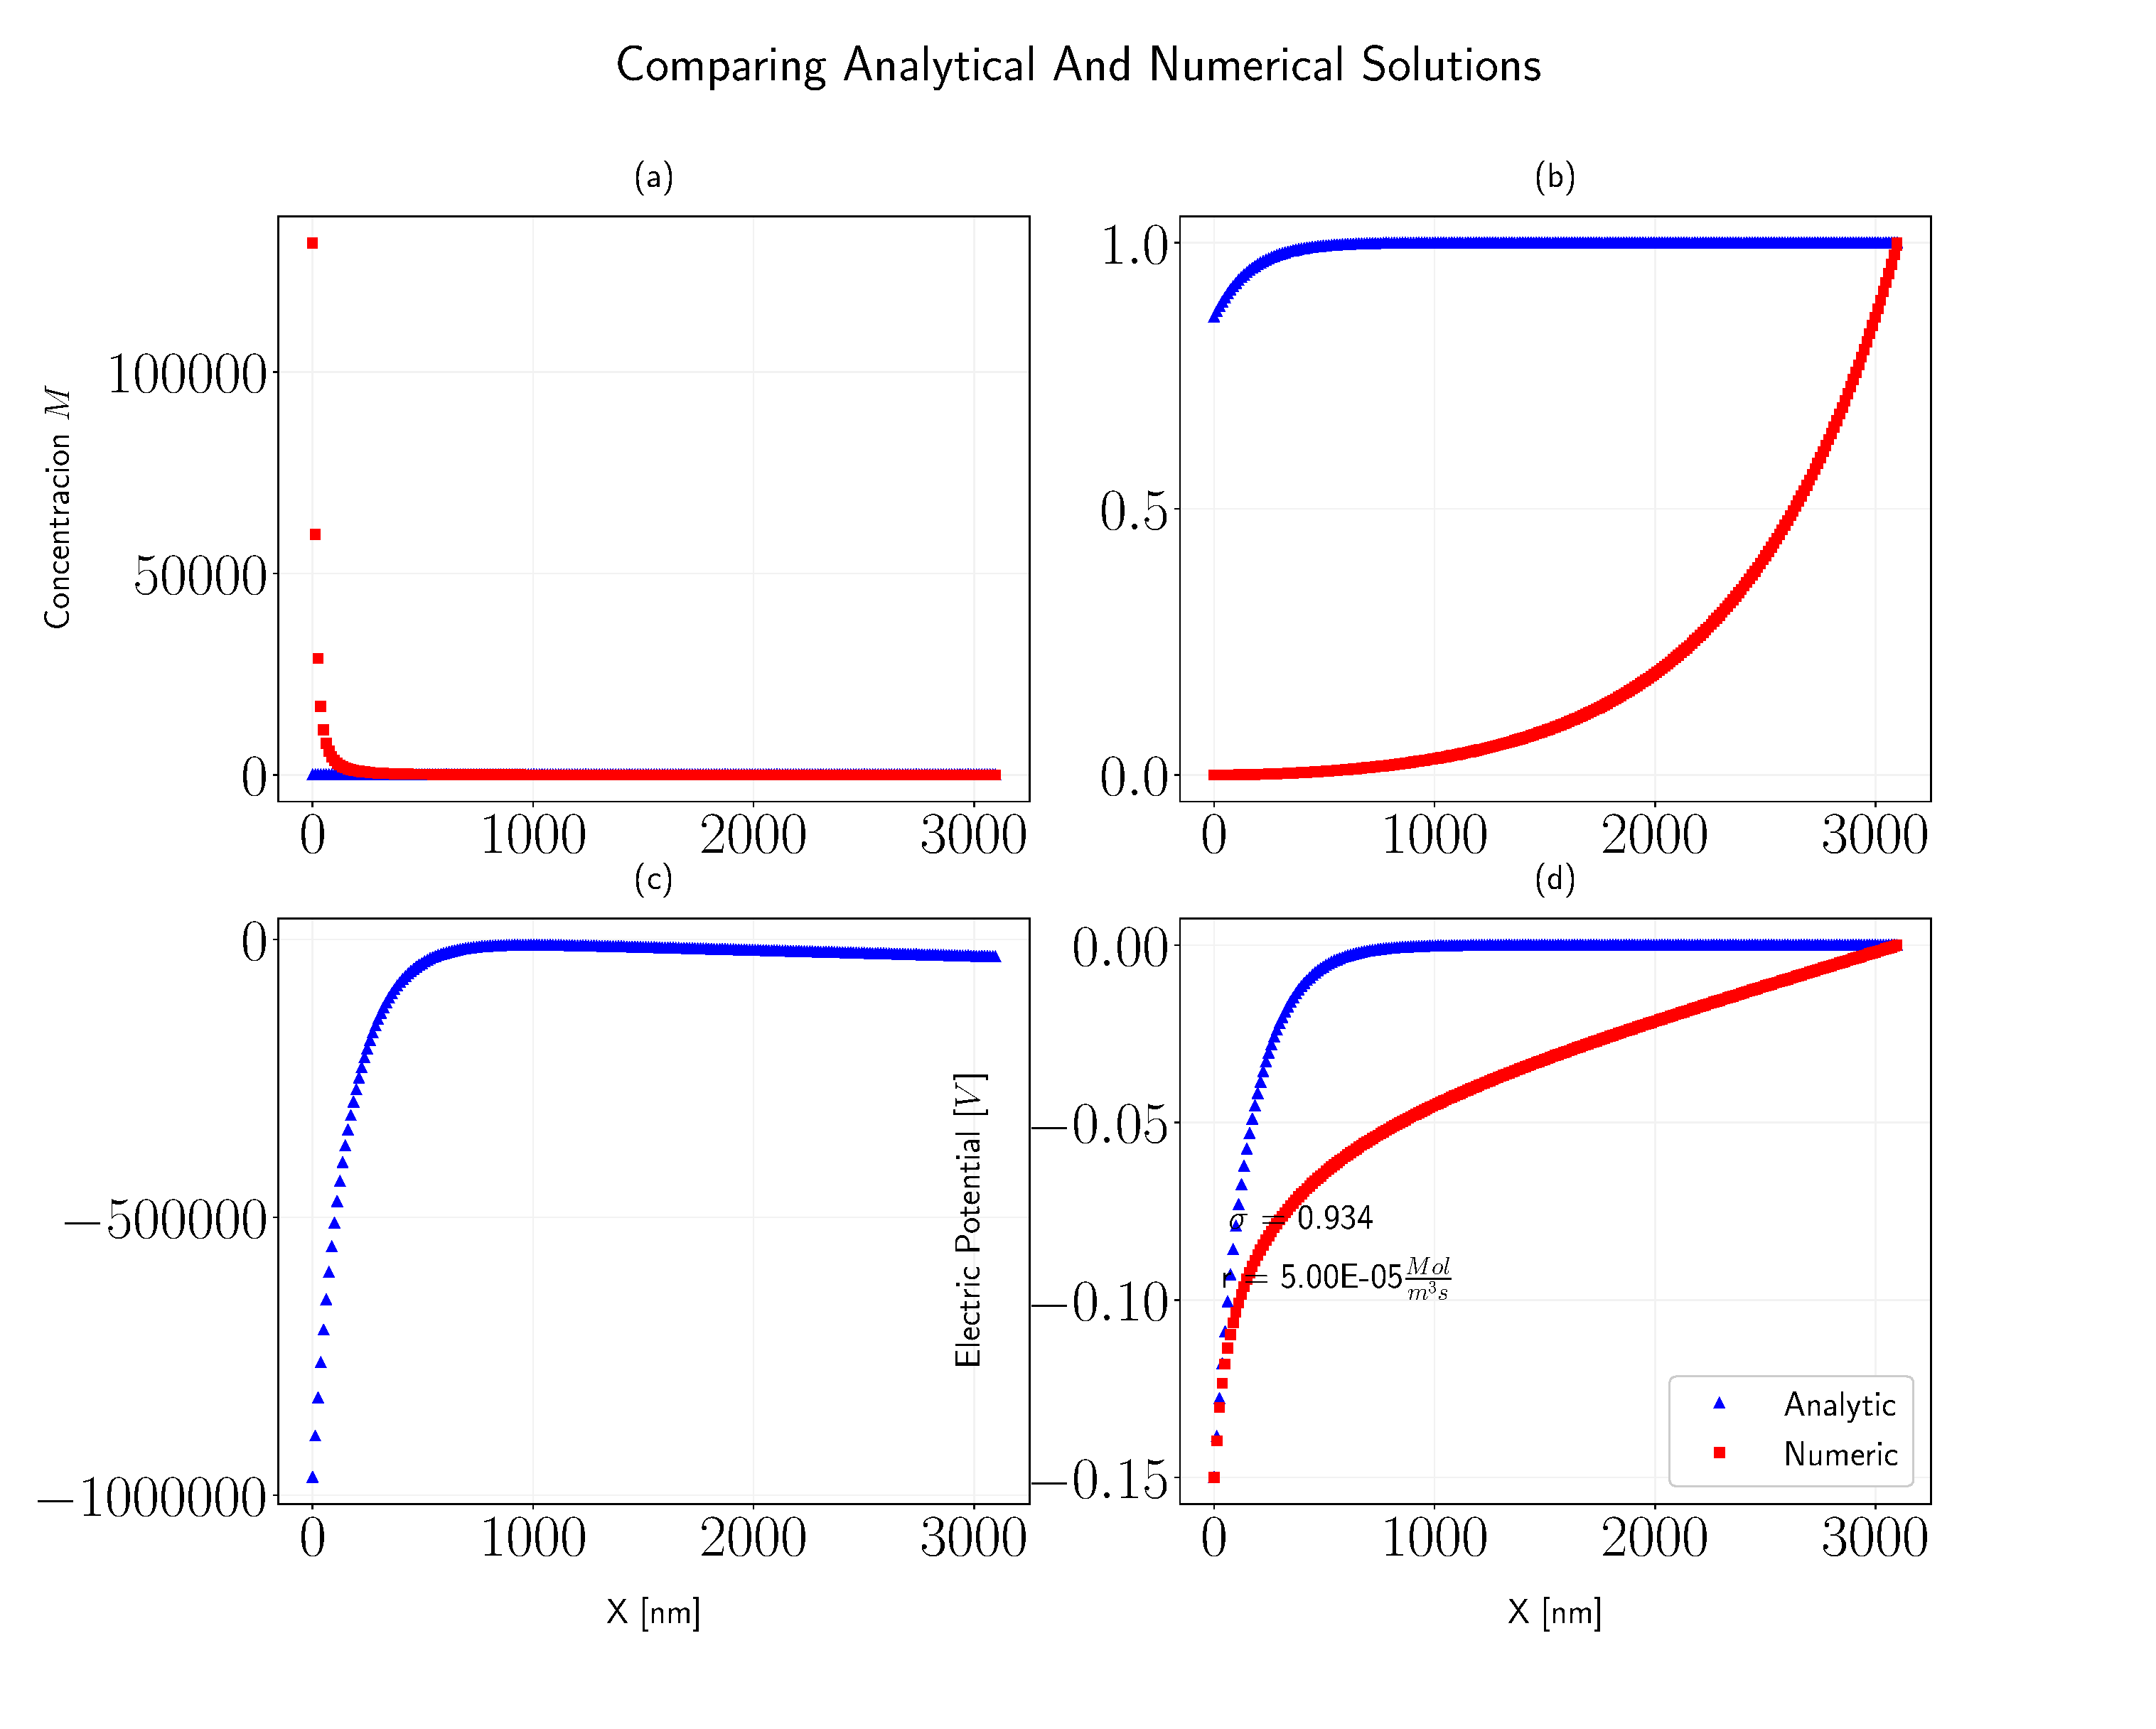
\includegraphics[width=\textwidth]{comparison0}
\caption{}
\label{fig:sub1}
\end{subfigure}%
\begin{subfigure}{.5\linewidth}
\centering
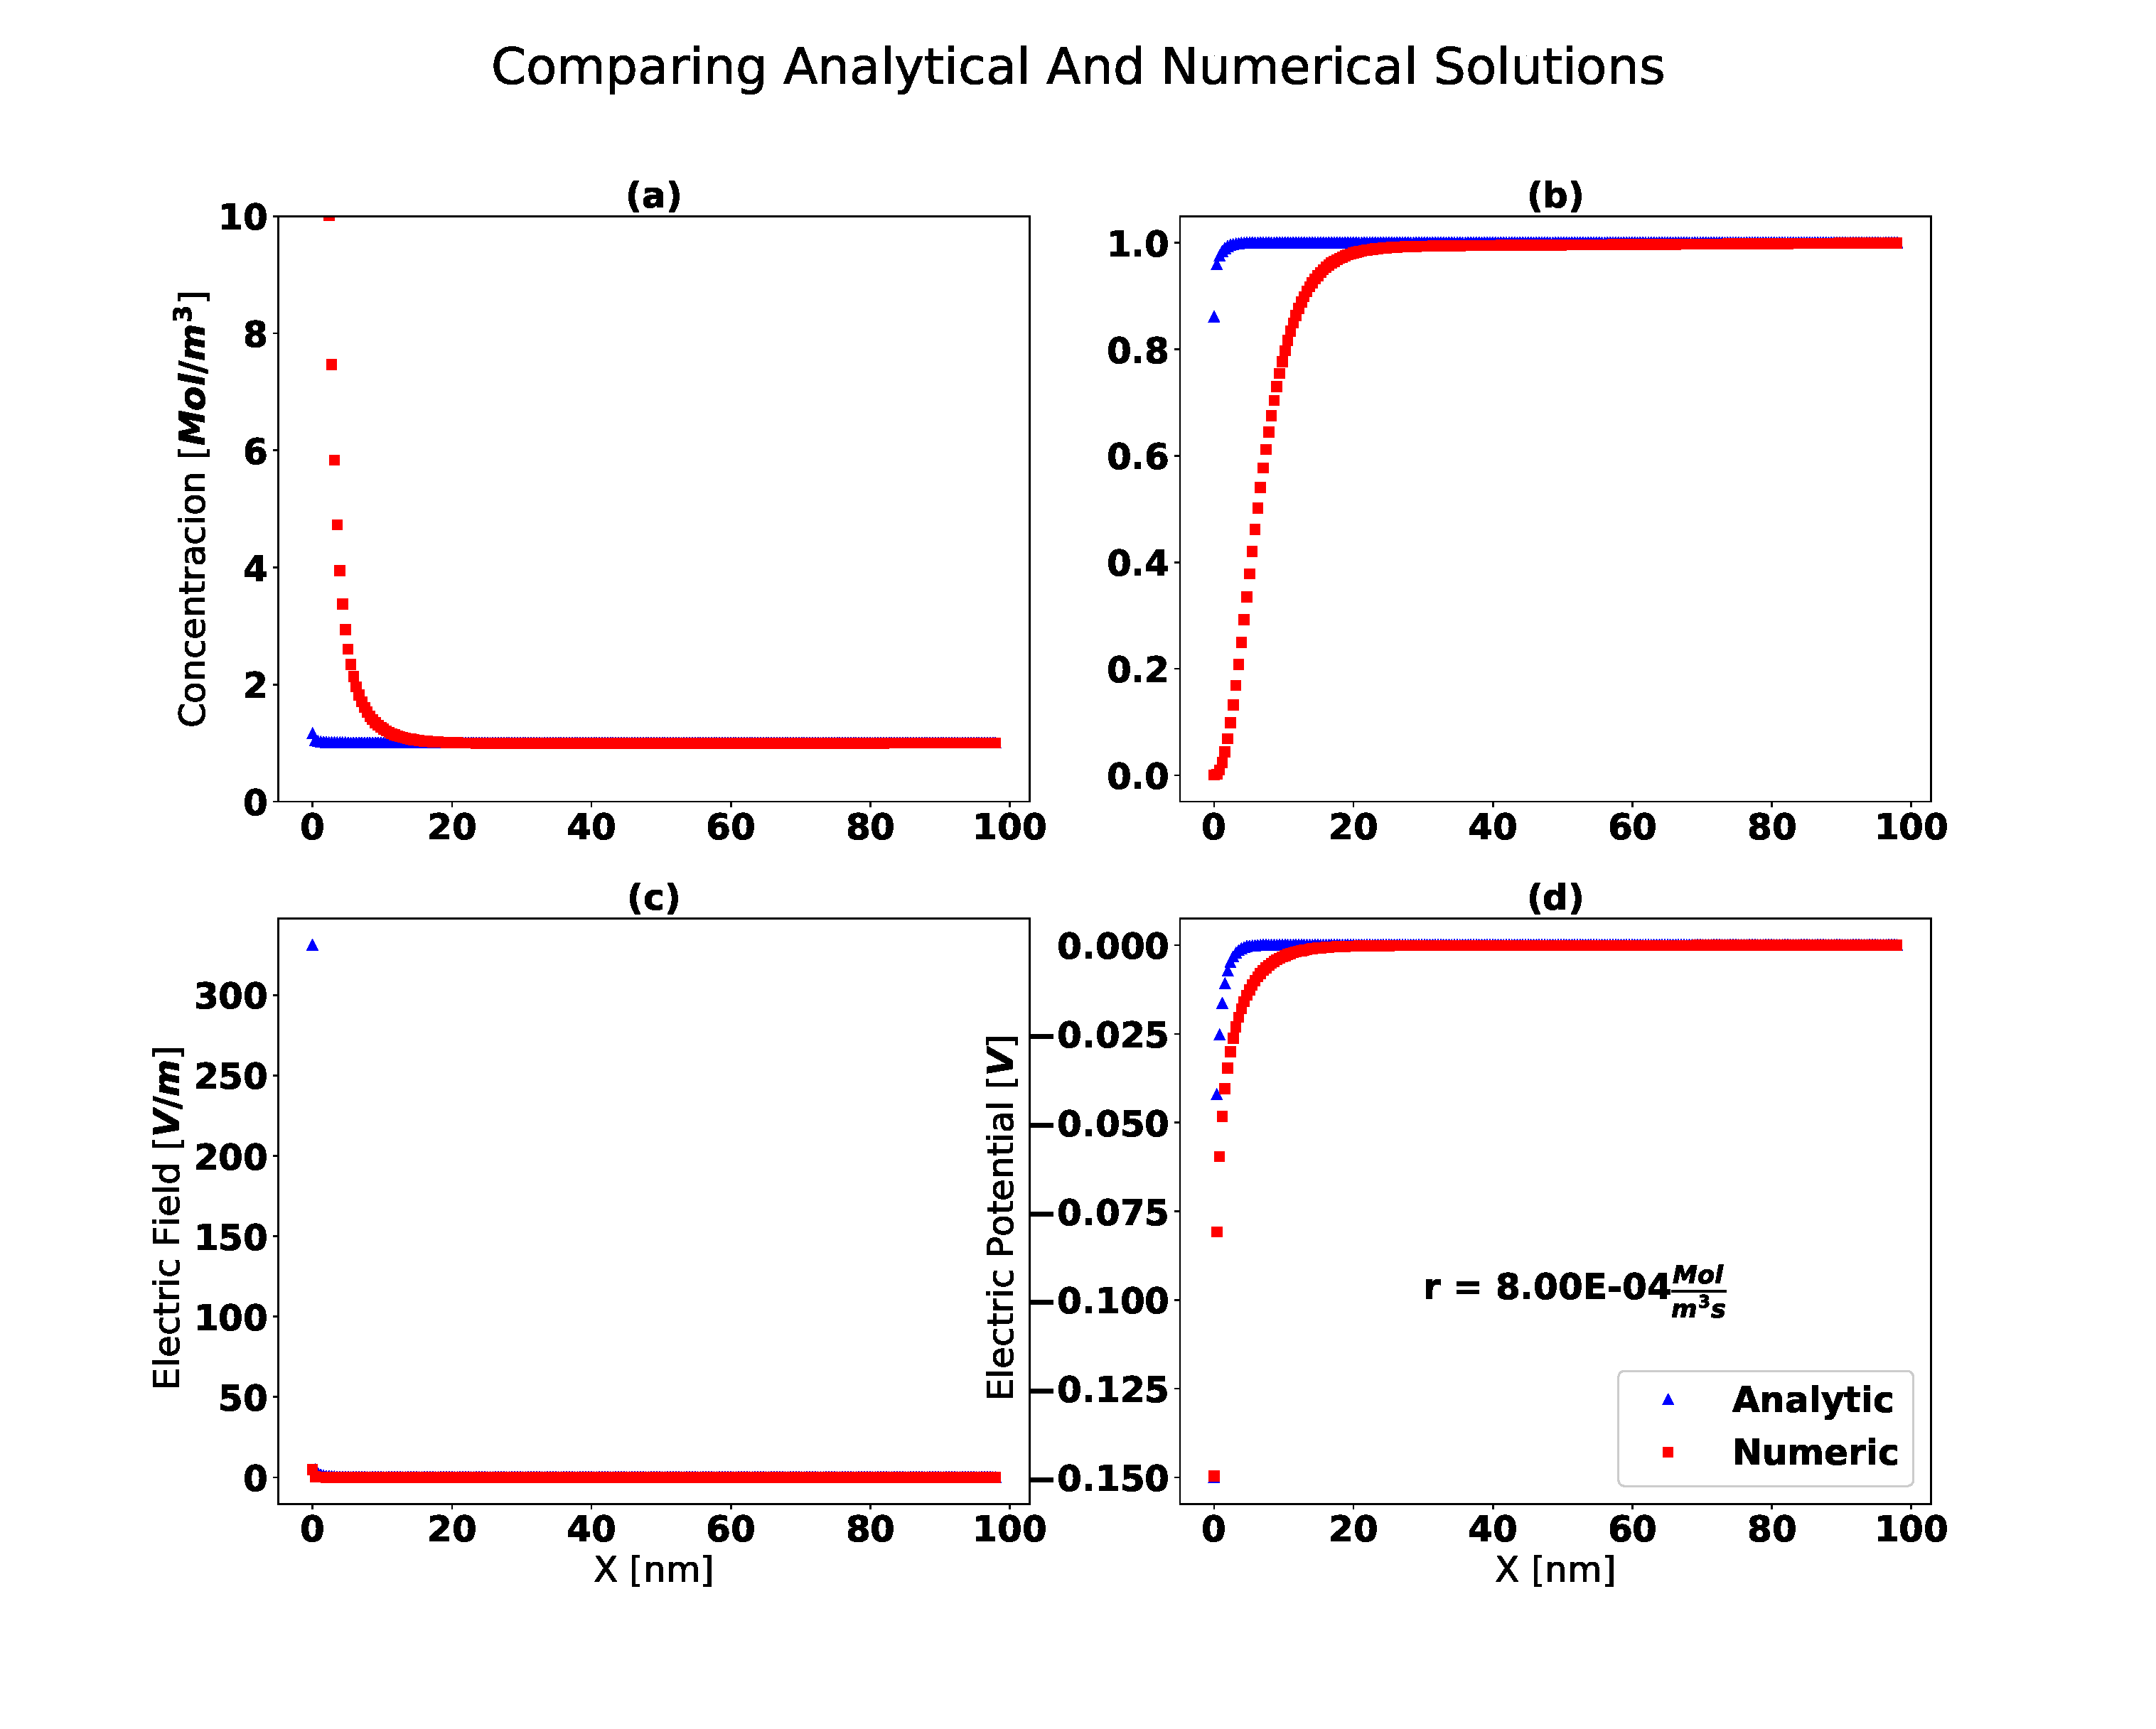
\includegraphics[width =\textwidth]{comparison1}
\caption{}
\label{fig:sub2}
\end{subfigure}\\[1ex]
\begin{subfigure}{\linewidth}
\centering
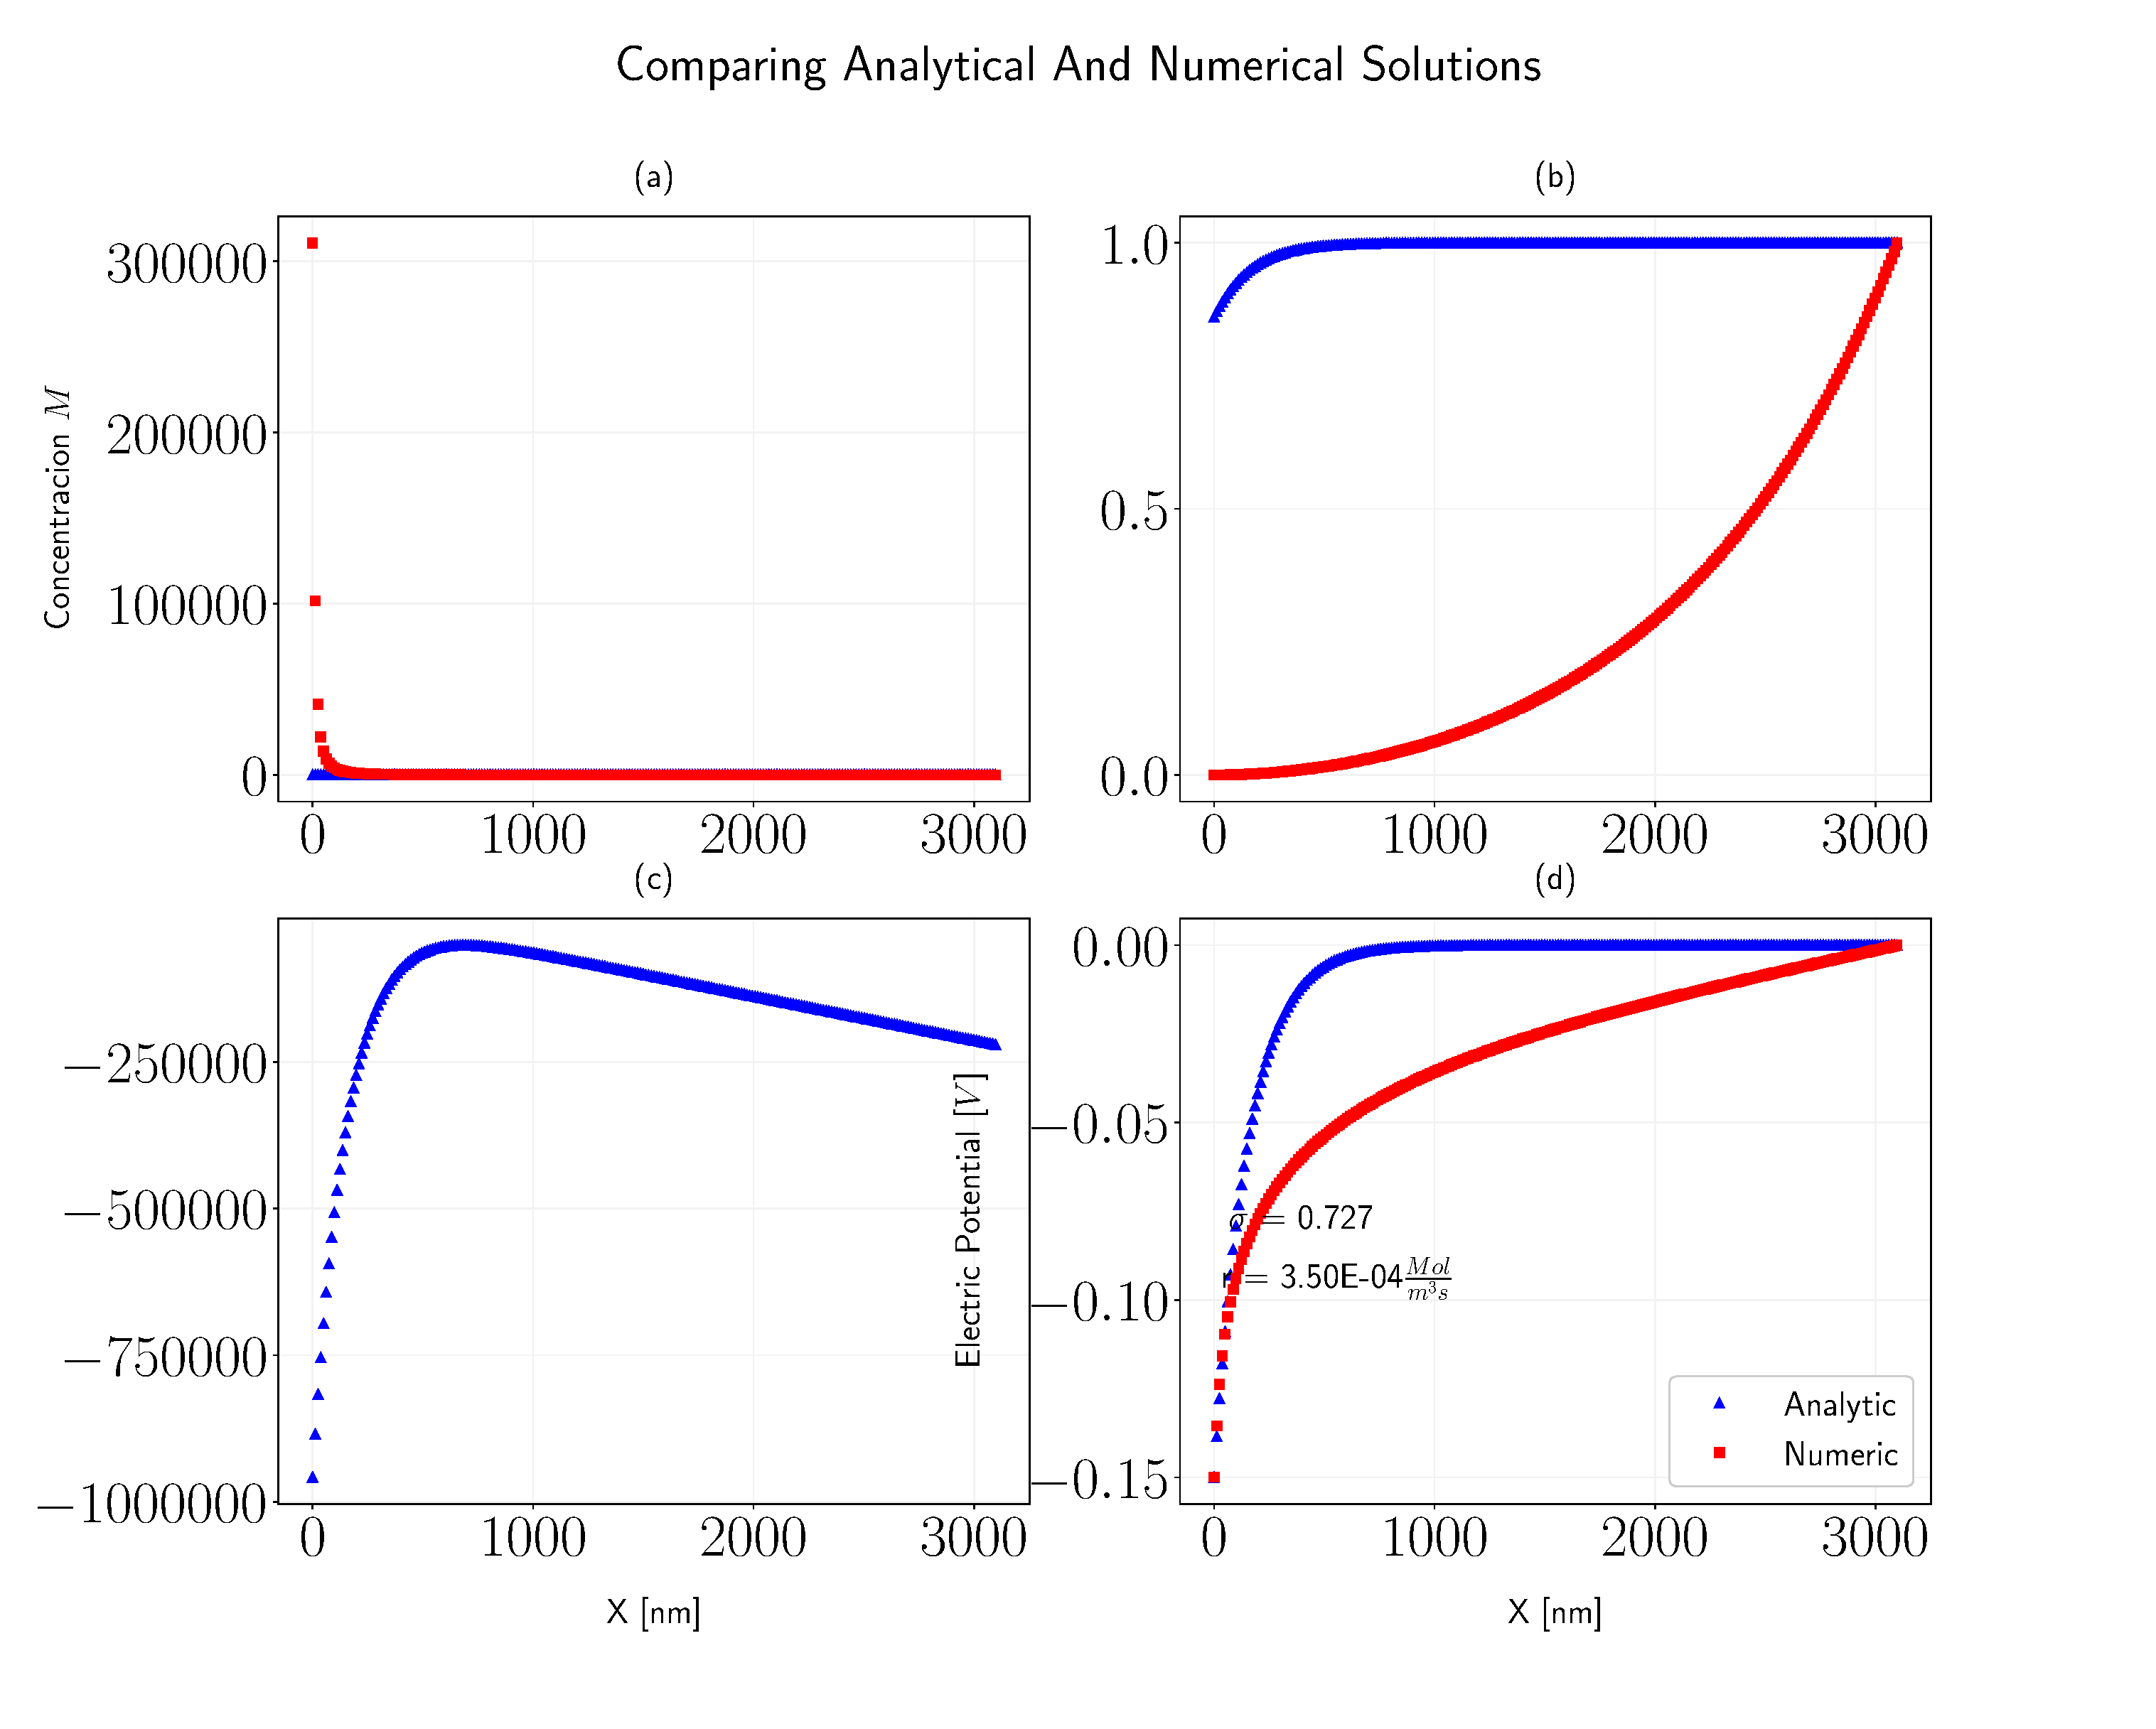
\includegraphics[width =0.5\textwidth]{comparison2}
\caption{}
\label{fig:sub3}
\end{subfigure}
\caption{Three subfigures}
\label{fig:comparison}
\end{figure}


